\section{Phương pháp nghiên
cứu}\label{sec:phuongphap}

\subsection{Biện minh lựa chọn thiết kế bán thực
nghiệm}\label{sec:bienminh}

Nghiên cứu này sử dụng phương pháp bán thực nghiệm (quasi-experimental)~\citep{shadishCook2002}
vì can thiệp kỹ thuật có thể được triển khai và đo lường, nhưng môi
trường thực nghiệm không thể được kiểm soát hoàn toàn. Một thực nghiệm
đúng nghĩa (true experiment) đòi hỏi phân bổ ngẫu nhiên, tài nguyên tính toán cố định, điều
kiện mạng ổn định, các lần chạy lặp lại trong trạng thái tài nguyên
giống hệt nhau và tập đối tượng tấn công đại diện cho thực tế. Những giả
định này không khả thi trong môi trường Databricks được sử dụng trong
nghiên cứu.

Thực nghiệm kiểm soát các yếu tố có thể kiểm soát được: cấu trúc
pipeline, seed sinh dữ liệu tổng hợp, danh sách kịch bản tamper, logic kiểm chứng, tập biến đo lường và thứ tự quy trình. Đồng thời, nghiên
cứu ghi nhận các yếu tố không thể kiểm soát: lập lịch trên nền tảng đám mây, trạng
thái khởi động, cache, độ trễ mạng và việc các kịch bản tamper là đại diện gần đúng (proxy)
do nhà nghiên cứu thiết kế, không phải mẫu ngẫu nhiên của không gian tấn công thực
tế. Vì vậy, kết quả được diễn giải là bằng chứng bán thực nghiệm về quan
hệ giữa điều kiện can thiệp và kết quả quan sát được, không phải kết luận nhân quả
phổ quát.

\subsection{Điều kiện can thiệp và điều kiện đối chứng}\label{sec:extra1}

Điều kiện can thiệp (treatment) là việc bổ sung Hash-linked Tamper-evident Ledger, lineage
recorder và bộ kiểm chứng vào một Data Pipeline chuẩn. Điều kiện đối chứng phụ thuộc vào câu hỏi nghiên cứu. Đối với phát hiện và truy vết, trạng thái pipeline sạch, không có kịch bản tamper, đóng
vai trò điều kiện đối chứng trước can thiệp. Đối với chi phí phát sinh, pipeline baseline không có
ledger và thành phần đo lường và kiểm chứng đóng vai trò điều kiện đối chứng
không tương đương.

\begin{figure}[t]
\centering
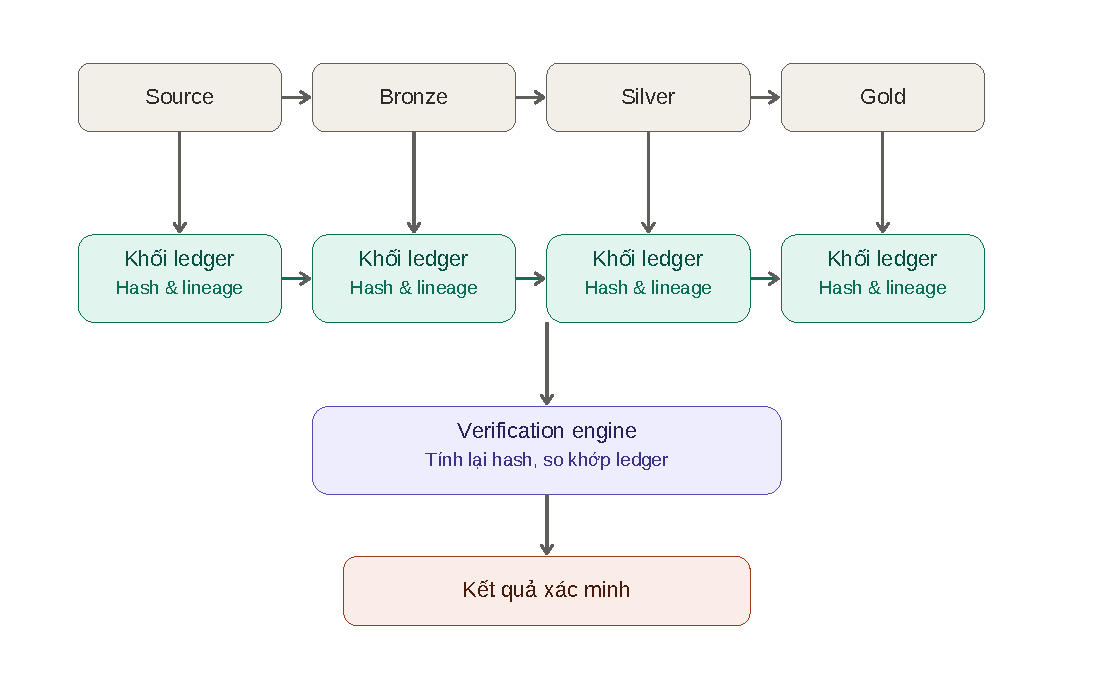
\includegraphics[width=\columnwidth]{images/kien_truc_ledger.pdf}
\caption{Hash-linked Tamper-evident Ledger cho Data Pipeline nhiều giai đoạn.}
\label{fig:architecture}
\end{figure}

\subsection{Giả thuyết nghiên cứu}\label{sec:giathuyet}

Tương ứng với bốn câu hỏi nghiên cứu, bốn giả thuyết được phát biểu
trong Bảng~\ref{tab:hypotheses}.

\begin{table}[!t]
\centering
\caption{Giả thuyết nghiên cứu}
\label{tab:hypotheses}
\begin{tabular}{|l|p{\dimexpr\columnwidth-1.2cm-6\tabcolsep\relax}|}
\hline
\textbf{Mã} & \textbf{Giả thuyết} \\
\hline
H1 & Treatment phát hiện tất cả kịch bản tamper được định nghĩa trước,
trong khi điều kiện sạch vẫn hợp lệ. \\
\hline
H2 & Treatment xác định được block sai lệch đầu tiên và liên kết được với
lineage event tương ứng. \\
\hline
H3 & Treatment làm tăng thời gian xử lý so với pipeline baseline, và
chi phí phát sinh thay đổi theo số lượng bản ghi. \\
\hline
H4 & Các biến không kiểm soát được khiến nghiên cứu không thể đưa ra kết
luận nhân quả mạnh như thực nghiệm đúng nghĩa (true experiment). \\
\hline
\end{tabular}
\end{table}
\subsection{Biến nghiên cứu}\label{sec:bienso}

Các biến độc lập gồm kịch bản tamper, số lượng bản ghi, giai đoạn pipeline,
cơ chế bảo mật và điều kiện chạy. Các biến phụ thuộc gồm kết quả kiểm chứng,
tỷ lệ phát hiện, độ chính xác của block sai lệch đầu tiên, mức độ đầy đủ
của truy vết, overhead bảo mật, thời gian chạy baseline, thời gian chạy có
cơ chế bảo vệ và thời gian kiểm chứng. Bảng~\ref{tab:variables} tóm tắt
các biến cốt lõi cùng loại và vai trò của chúng.

\begin{table}[!t]
\centering
\footnotesize
\caption{Các biến thực nghiệm cốt lõi}
\label{tab:variables}
\begin{tabular}{|p{1.9cm}|p{1.4cm}|p{3.9cm}|}
\hline
\textbf{Biến} & \textbf{Loại} & \textbf{Vai trò} \\
\hline
Kịch bản tamper & IV phân loại & Tác nhân kiểm thử phát hiện và
truy vết. \\
\hline
Số lượng bản ghi & IV thứ bậc & Yếu tố đánh giá mức thay đổi chi phí theo quy mô dữ liệu. \\
\hline
Giai đoạn pipeline & IV phân loại & Ngữ cảnh cho block và ánh xạ lineage. \\
\hline
Cơ chế bảo mật & IV nhị phân & So sánh control và treatment. \\
\hline
Kết quả kiểm chứng & DV phân loại & Kết quả phát hiện chính. \\
\hline
Tỷ lệ phát hiện & DV số & Tỷ lệ kịch bản tamper được phát hiện. \\
\hline
Overhead thời gian chạy & DV số & Chi phí thời gian bổ sung của treatment. \\
\hline
\end{tabular}
\end{table}

\FloatBarrier
